\documentclass[]{usiinfbachelorproject}
\captionsetup{labelfont={bf}}
\usepackage{color, colortbl}
\usepackage{float}
\usepackage{longtable}
\usepackage{tabu}
\usepackage{listings}
\lstdefinelanguage{json}{
    showstringspaces=false,
    breaklines=true,
    frame=lines
    basicstyle=\scriptsize,
}
\definecolor{LightCyan}{rgb}{0.88,1,1}
\definecolor{LightGreen}{rgb}{0.65,0.83,0.56}

\author{Stefano Peverelli}
\title{Using Machine Learning and Simulation to predict the traversability of a given terrain by a simple robot}
\versiondate{\today}
\begin{committee}
%With more than 1 advisor an error is raised...: only 1 advisor is allowed!
\advisor[Universit\`a della Svizzera Italiana, Switzerland]{Prof.}{Luca Maria}{Gambardella}
%You can comment out  these lines if you don't have any assistant
\assistant[Universit\`a della Svizzera Italiana, Switzerland]{PhD}{Alessandro}{Giusti}
\assistant[Universit\`a della Svizzera Italiana, Switzerland]{PhD}{Jerome}{Guzzi}
\end{committee}
\abstract{
Autonomous vehicles in unstructured outdoor environment need to estimate the \textit{traversability} of the terrain. \\ %TODO cite traversability
This thesis presents a new approach based on simulation and machine learning to predict whether a given 3D region is traversable by a simple ground robot.\\
The proposed approach has two main phases: the first consists of simulating a robot that traverses a 3D terrain in a virtual environment, determine in which areas it got stuck or capsized, 
and collect data from the simulations to obtain an extensive dataset of possible outcomes.
The second phase instead aims to analyze the resulting dataset and use it to train a neural network model, whose purpose is, to judge the traversability
of a terrain (by its 3D structure), and plan a path the robot can traverse. \\
By using an approach based on machine learning, there's no need to manually define heuristic
rules to predict the traversability of terrain patches; moreover, the approach is applicable to any type of ground robot (wheeled/legged) as long as it can be reliably simulated.
}
\begin{document}
\maketitle
\tableofcontents
\newpage
%%%%%%%%%%%%%%%%%%%%%%%%%
\section{Introduction} \label{introduction}
Robot navigation in outdoor environments is a very challenging task, as traversability is a really complex function of both terrain features and robot characteristics.
This thesis approaches terrain scoring from a machine learning perspective: the proposed method uses a robot's experience in navigating the environment to train a
classifier. \\
Data collection is achieved in a virtual environment, which offers a good and cheap starting point, despite of certain limitations, such as numerical approximation and the inability to resemble
vegetation or sloping ground. \\
A main assumption of this approach is that a terrain map is available at priori (e.g. 3D radar surface reconstruction). \\
Each simulation consists of a challenge for the robot, which, starting from an initial random point, needs to follow a predetermined path to reach a goal point. For convention we will call the
square area given by the path a \textit{patch}.
The patch itself contain a lot of information about the terrain surface the robot has dealt with, steepness or presence of peaks and depressions, thus from the patch we then compute some
statistics that the classifier will use during its training.\\
The evaluation of the quality of predictions made by the classifier, is performed by computing the area under the \textit{receiver operating characteristic} (ROC) curve, which features both true positive
and false positive rates; this evaluation phase is tested for several linear methods, and all scores are presented in the Evaluation and Results section.
%%%%%%%%%%%%%%%%%%%%%%%%%
\subsection{State of the Art}
Previous research has addressed the problem of estimating traversability for ground robots in outdoor environments, following different approaches.\\
Nowadays, thanks to the progress made by 3D vision sensors, a common trend is to combine acquired RGB-D images to machine learning techniques, for terrain traversability assessment.\\\\
A solution in this direction is proposed in \cite{Kim}; the authors presents a new framework for online-learning achieved by the correspondence between vehicle's navigation experience and
visual terrain data. \\
Navigation experience such successful traverses, or collisions is assessed by robot's on-board sensors like (IMU \cite{imu}), while terrain data is labeled as traversed or not
by stereo imagery; automatic labeled data is then passed in input to an online classifier that trains incrementally as the robot navigates the environment. \\\\
Another example of the use of RGB-D images acquired by \textit{time of flight cameras} is presented in \cite{tofc}. \\
The proposed method analyze and segments RGB data streams into group pixels
belonging to the same physical object. Then from the depth data stream, it estimates the ground plane (by computing the \textit{v-disparity} \cite{raphael}) to obtain a first measure of
traversability. From this first estimation, an arbitrary number of pixels with an high probability of belonging to the ground plane is considered, and for each of pixel, a scoring function is computed.\\\\
Another work that relies on the acquisition of RGB-D images is the one presented in \cite{bellone}. Interesting is the introduction of a novel 3D descriptor, the (UPD) \textit{uneveness point descriptor},
that observes the distribution of surface's normal vector directions using (PCA) \cite{pca} to score terrain features and detect obstacles.\\\\
The main difference between these approaches and our work is the use of simulation combined with machine learning. As virtual simulation environments are becoming more realistic and powerful,
they offer a good compromise to acquire data in a cheap, but reliable way. Moreover, this approach can be tested on any type of robot (at no additional cost), as long as it can be
accurately simulated.




\newpage
%%%%%%%%%%%%%%%%%%%%%%%%%
\section{Project requirements and analysis}
%%%%%%%%%%%%%%%%%%%%%%%%%
\subsection{Learning of traversability}
In order to exploit machine learning techniques to create trained models that can judge the traversability of a given terrain, a dataset of terrain features has to be generated.
Obtaining a dataset in the real world requires a lot of time and specific tools, instead a proper simulation environment is better suited. Among various
robot simulation platforms we have chosen V-REP \cite{vrep}. V-REP offers a complete simulation environment that includes physics and
robot terrain interactions. In the next section the basic structure of the framework is presented.
\subsection{Simulation}
\begin{figure}[h]
\minipage{0.32\textwidth}
  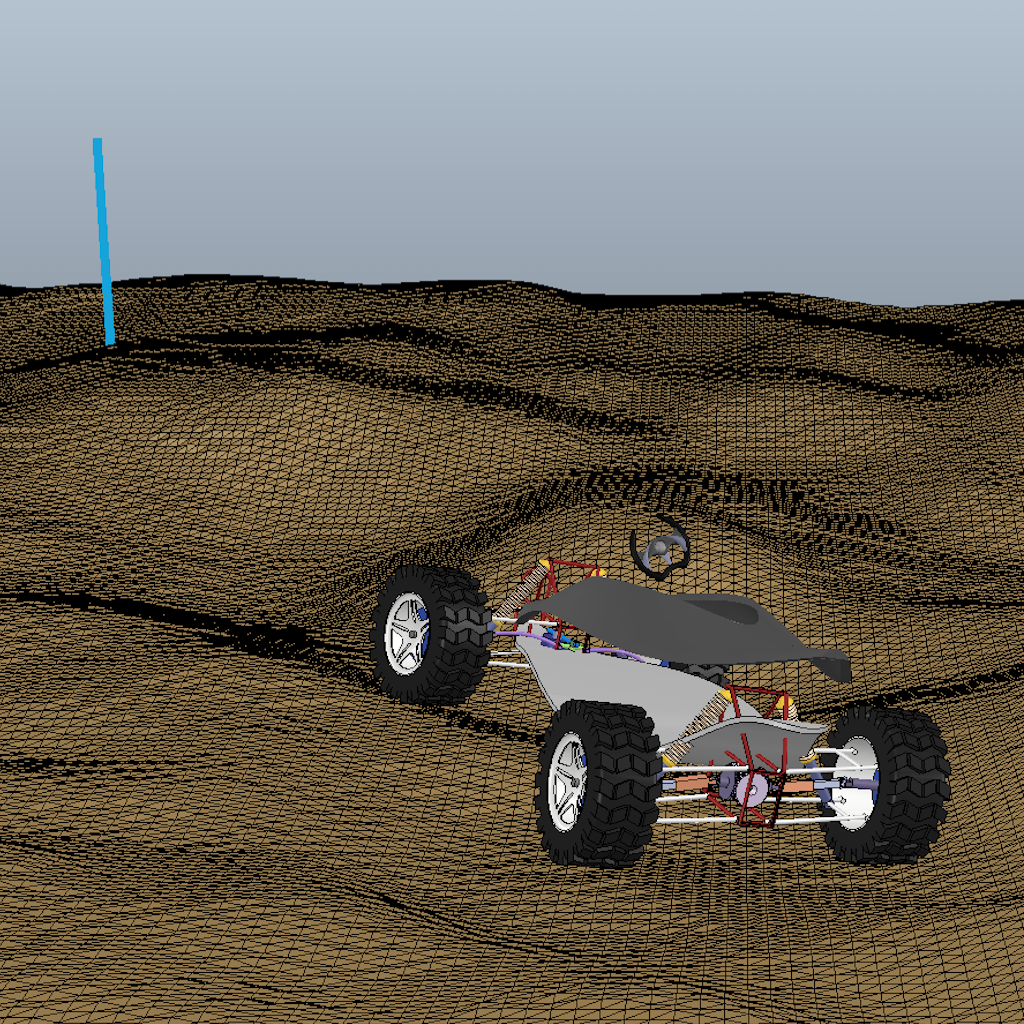
\includegraphics[width=\linewidth]{simulation}
    \caption{The robot approaching the goal point}\label{fig:simulation}
\endminipage\hfill
\minipage{0.32\textwidth}
  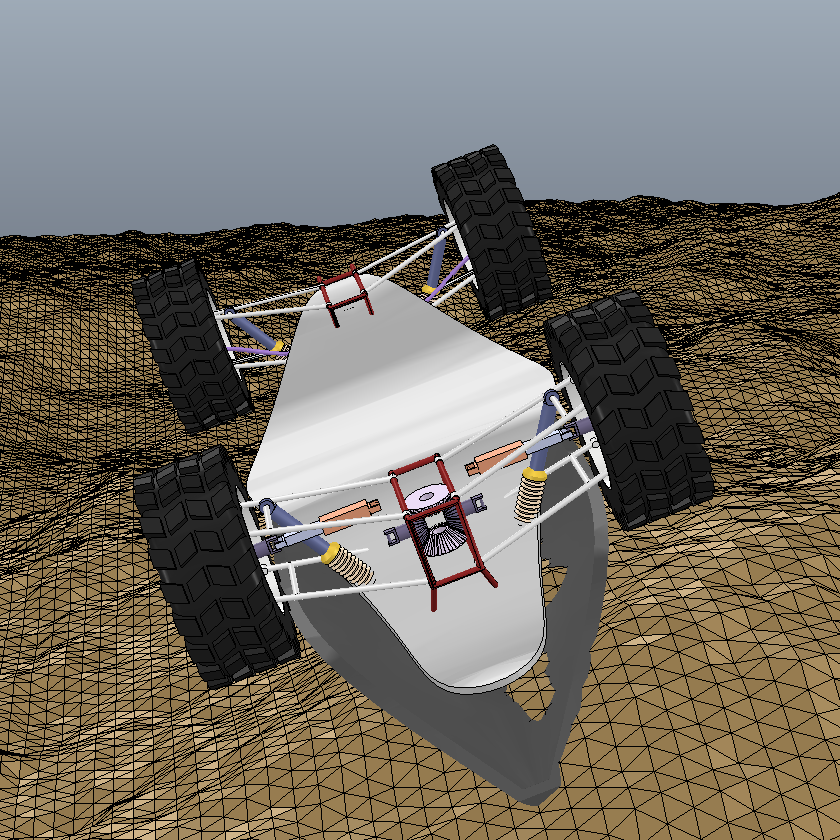
\includegraphics[width=\linewidth]{capsized}
    \caption{A possible scenario, a capsized robot}\label{fig:capsized}
\endminipage\hfill
\minipage{0.32\textwidth}
  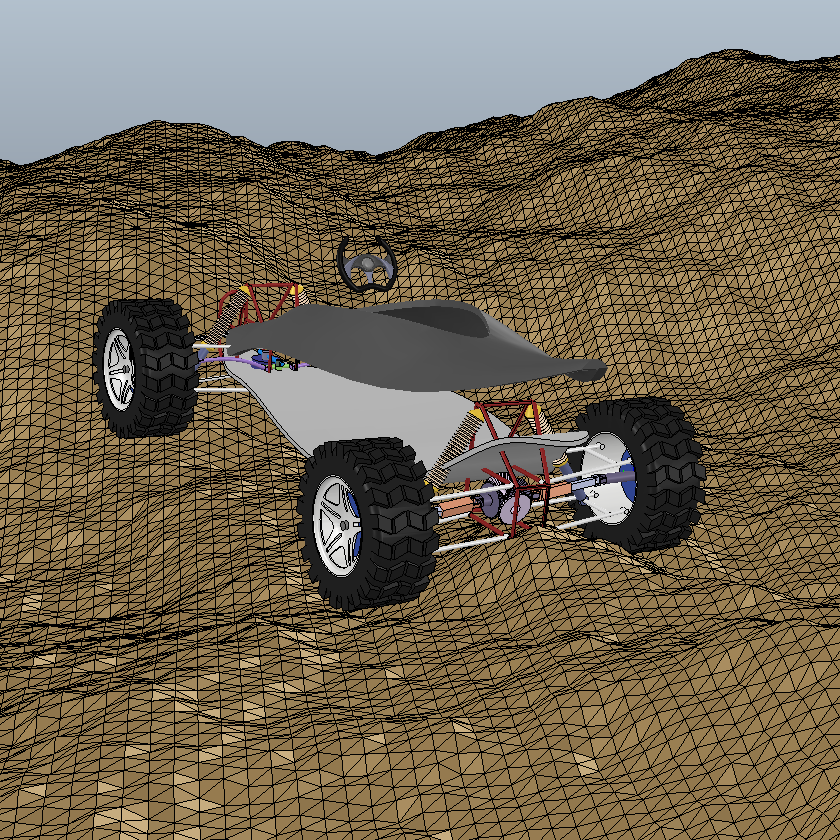
\includegraphics[width=\linewidth]{stuck}
    \caption{A possible scenario, a stuck robot}\label{fig:stuck}
\endminipage\hfill
\end{figure}
\noindent
The general idea behind the simulation is to place a robot on a terrain moving towards a goal point, and to stop it when a break condition happens: either the robot has
reached the goal point or it has failed to. In order to ensure this boolean condition a time limit has to be decided; thus a stuck or capsized robot will
result in a failed attempt. \\
At each simulation time step specific data is computed, like the robot's ideal trajectory, yaw and position; the main reason behind the recording of these data
is that the robot needs to be guided to the goal point, so it needs its steer to be corrected while encountering terrain irregularities.
Eventually, data such as the goal point position, robot's initial and final position, elapsed time and success or failure, are saved into a CSV file. In order to simulate different
scenarios, robot's velocity and distance to the goal can be passed via input to the script that handles the simulations.

\subsection{Terrain Generation}
\begin{figure}[h]
\minipage{0.3\textwidth}
  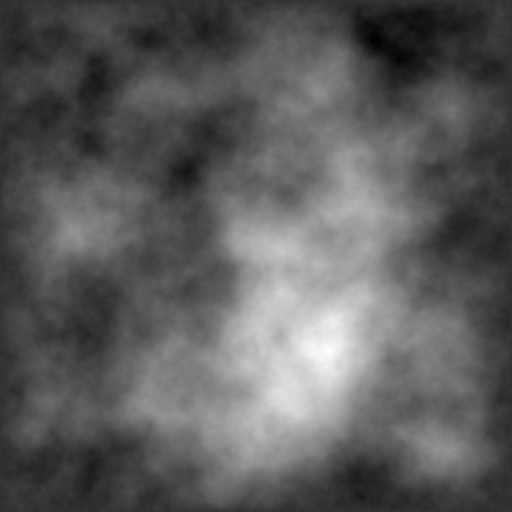
\includegraphics[width=\linewidth]{2dterrain}
    \caption{An example of generated heightmap}\label{fig:2dterrain}
\endminipage\hfill
\minipage{0.6\textwidth}
  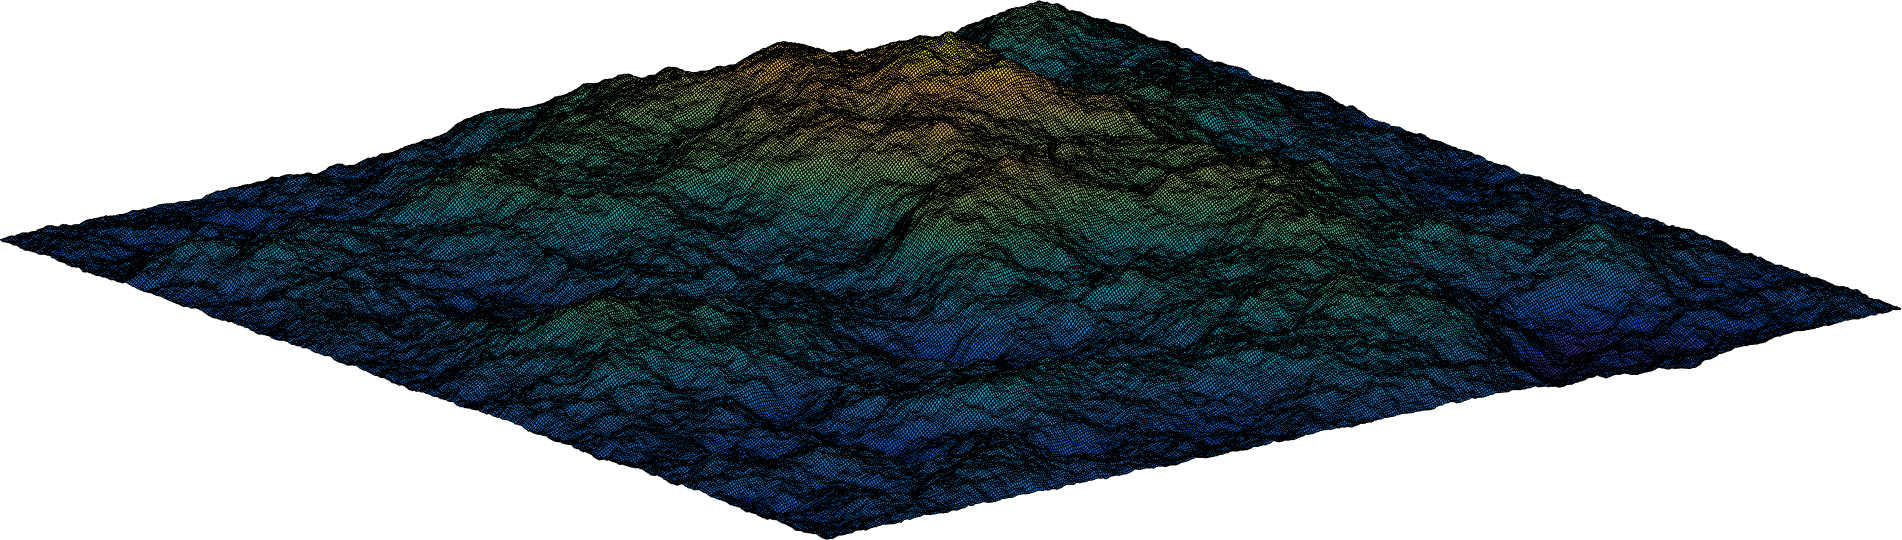
\includegraphics[width=\linewidth]{3dterrain}
    \caption{The corresponding 3D terrain}\label{fig:3dterrain}
\endminipage\hfill
\end{figure}
\noindent
When simulating a virtual environment, reality must be resembled as much as possible, thus one must be as precise as possible when generating rough terrains.
The task of creating random but meaningful and realistic terrains can be accomplished using just random noise and the \textit{Gaussian blur} function, which create \textit{heightmaps} that are then extruded
to 3D terrain.

\subsection{Data postprocessing}
\begin{figure}[h]
\minipage{0.7\textwidth}
  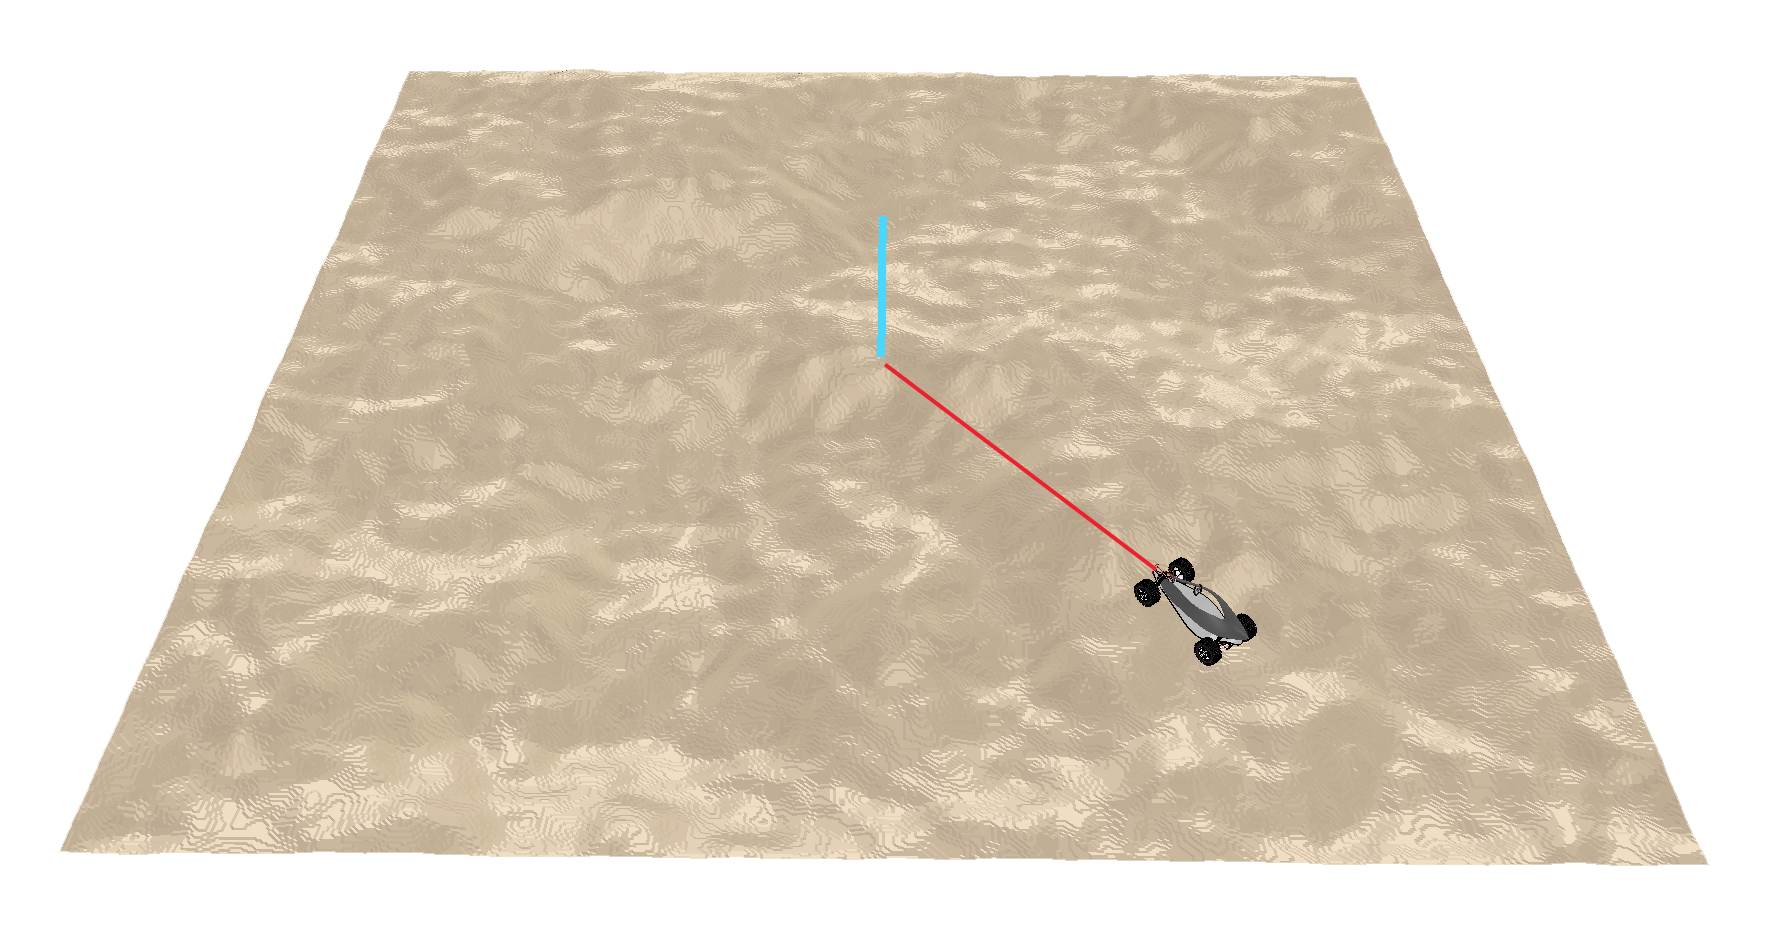
\includegraphics[width=\linewidth]{3Dsim}
    \caption{Simulation scenario: robot(1m x 0.5m x 0.4m) is placed in an initial random position (x,y) with a goal point at distance d (in this case d=4m), on a 10x10m heightmap.
             In red is highlighte the ideal path the robot will try to follow to reach the goal.}\label{fig:3Dsim}
\endminipage\hfill
\minipage{0.28\textwidth}%
  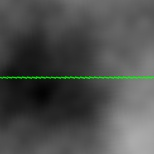
\includegraphics[width=\linewidth]{rpatch}
  \caption{The cropped and rotated patch we have extracted from the robot's navigation, from which we compute the set of feature for the training dataset}\label{fig:rpatch}
\endminipage
\end{figure}
\noindent
In order for a classifier to actually learn to judge a given terrain, we need to extract some features from each patch that comes out from the simulations in a post-processing phase.\\
The concept for which a patch is traversable, strictly depends on the direction taken into account, thus the need to perform a roto-translation of each patch, so that only one direction
is taken into account (from west to east).
From each rotated patch then we compute the following statistics: mean, variance, mean and variance of the gradient of $x$, and mean and variance of the gradient of $y$. These are the features
that compose the actual dataset.

\subsection{Classification}
Classification is the process that exploits what learned from labeled data and tries to predict the class of unlabeled data; labeled data is simply the training dataset
obtained from the simulations and the post-processing phase, and unlabeled data are the features extracted in a post-processing phase from a testing heightmap.
In order to build and test a trained model, we have chosen scikit-learn \cite{scikit-learn}, a python based framework for machine learning.\\
Supervised learning in scikit is very straightforward; it offers a variety of linear models to work with, so there's no need to actually build a classifier from scratch.

\subsubsection{Learning algorithms}
For the learning process several algorithms were taken into account, from support vector machines to logistic regression, eventually focusing on this last one, which is better suited
when investigating a dichotomous behavior.

\subsubsection{Logistic regression}
Logistic regression is a \textit{regression model} to estimate the probability of a binary response based on one or more independent variables.
The main goal of logistic regression is to find the best fitting model between the set of independent variables (features) and the binary characteristic of interest (target) using a logistic
function. \\
The logistic function ${\displaystyle \sigma (t)}$ [Figure~\ref{fig:logisticfunction}] is defined as follows:
\begin{equation}
    \sigma (t) = \dfrac{e^t}{e^t + 1} = \dfrac{1}{1 + e^{-t}}
\end{equation}
where $t$ is a linear combination of multiple explanatory variables:
\begin{equation}
    t = \beta_0 + \beta_1x
\end{equation}
\noindent
In order to estimate the probability then, one must first estimate the coefficients. Unlike linear regression, where parameters are estimated using the method of least squares, in logistic
regression they are estimated by using the \textit{maximum likelihood estimation} method \cite{mle}. While it is possible to apply linear regression to estimate the probability, the result
would be an unbounded measure, instead with logistic regression, the estimation is guaranteed to be inside the closed interval $[0,1]$.
\clearpage
\section{Project Design}
% In this section the implementation of previously described components is presented.

\subsection{Simulation and Data Collection}
\begin{figure}[h]
\minipage{0.5\textwidth}
    V-REP offers a variety of choices on how to interface with its core features. Figure~\ref{fig:vrep} shows the main V-REP's architecture.\\
    The are four main ways to access V-REP functionalities:
\begin{itemize}
    \item the regular API
    \item the remote API
    \item the ROS \cite{ROS} interfaces
    \item the auxiliary API
\end{itemize}
For this work we have chosen the regular API. The regular API is composed by several hundreds of features which can be invoked from C/C++ application or extended by custom lua functions.
Since the main client application provides a simple way to handle the simulation by controlling the main script, the chosen approach was to only extend the desired functionalities by writing
lua code. As mentioned in the previous section, the robot needs to be guided towards the goal point, thus the need for writing a controller.
\endminipage\hfill
\minipage{0.45\textwidth}
  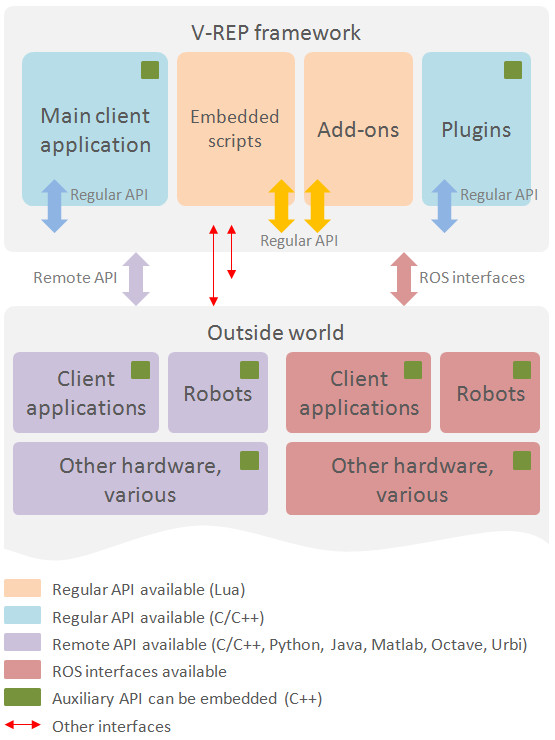
\includegraphics[width=\linewidth]{vrep}
    \caption{The V-REP API framework}\label{fig:vrep}
\endminipage\hfill
\end{figure}

\subsubsection{The robot model and its controller}
\begin{figure} [h]
\centering
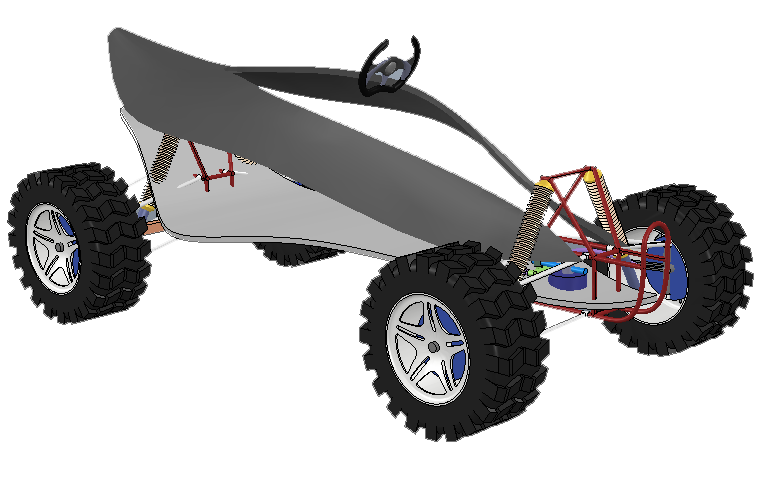
\includegraphics[width=0.5\textwidth]{robot}
    \caption{The "Manta with differential" model (courtesy of Qi Wang)}
\label{fig:robot}
\end{figure}
\noindent
We used the robot model shown in Figure~\ref{fig:robot}; it was chosen as a simple but also ideal representation of an off-road vehicle.\\
In V-REP each model has its own associated script which describes its behavior during simulation. Each script is composed by three main parts such initialization, actuation and cleanup phases. \\
The initialization phase is executed just once (when the simulation starts) providing a safe environment to initialize parameters like maximum time per simulation, motor velocity, maximum steer
angle and more others.  Table~\ref{table:params} lists the core parameters and corresponding values used.\\
The actuation part gets executed at each simulation time step ($dt = 50ms$) and is the core of each script, in which the actual behavior of the model is described. \\
Thus each $50ms$ robot's direction is checked, and if necessary, corrected; this process is repeated until either the maximum time per simulation has elapsed, or the robot is in the
area of interest of the goal point. At this point all necessary data is saved into a CSV file as shown below. \\\\
\begin{longtabu}{| c | c | c | c | c | c |}
\rowfont{\bfseries}
    \hline
    TRAVERSED & ELAPSED\_TIME(s) & GOAL(x,y) & R\_I(x,y) & R\_F(x,y) \\
    \hline
    \rowcolor{LightGreen}
    1 & 2.90 & 0.61, -0.40 & 0.58, -0.10 & 0.60, -0.35 \\
    \rowcolor{LightGreen}
    1 & 3.05 & 0.79, -0.79, & 0.52, -0.66 & 0.73, -0.77\\
    0 & 10.00 & 0.38, -0.56 & 0.64, -0.70 & 0.55, -0.63\\
    0 & 10.00 & 0.47, -0.51 & 0.71, -0.70 & 0.55, -0.55\\
    0 & 10.00 & 0.61, -0.25 & 0.34, -0.13 & 0.33, -0.13\\
    \rowcolor{LightGreen}
    1 & 5.05 & 0.78, -0.15 & 0.62, -0.41 & 0.77, -0.18\\
    0 & 10.00 & 0.61, -0.14 & 0.62, -0.44 & 0.61, -0.23\\
    0 & 10.00 & 0.68, -0.41 & 0.70, -0.71 & 0.67, -0.49\\
    0 & 10.00 & 0.82, -0.15 & 0.72, -0.43 & 0.77, -0.20\\
    0 & 10.00 & 0.21, -0.53 & 0.48, -0.66 & 0.50, -0.62 \\
    \hline
\caption{Instance of data saved from the simulations}
\label{table:datasim}
\end{longtabu}
\noindent
The first column identifies whether the robot has reached the goal point or not, the second is just the elapsed time in seconds, the third column represents the screen coordinates of the goal point,
and the last two columns, the robot initial and final screen coordinates.
\begin{table}[H]
\scriptsize
\centering
\begin{longtabu}{| c | c | c | c | c |}
\rowfont{\bfseries}
    \hline
    MAX\_SIM\_TIME(ms) & MOTOR\_VEL & MAX\_STEER\_ANGLE(in $^{\circ}$) & AREA\_OF\_INTEREST(radius in m) & DIST\_TO\_GOAL(in m)\\
    \hline
    10'000 & 1.0 & 30 & 0.2 & 3.0\\
    \hline
\end{longtabu}
\caption{Default values for robot parameters}
\label{table:params}
\end{table}
\subsubsection{The main script}
\noindent
In order to run a simulation, V-REP needs a scene object; this is the place where all required objects are displayed. The first task is to load a heightmap into a new scene, this can be easily done
from the main menu, or via the API, although only \textit{collada} and \textit{wavefront} objects are currently supported.\\
Once the heightmap is extruded to a 3D terrain, that's when the main script gets executed. In the initialization phase the robot model is loaded an positioned in a random position onto the
heightmap. Then the goal point is placed in the direction of the robot ad a distance $d$ (defined via input).
As the simulation is handled by the robot's script, the main script does not do anything in its actuation phase.
\subsection{Terrain Generation}
\begin{figure} [h]
\centering
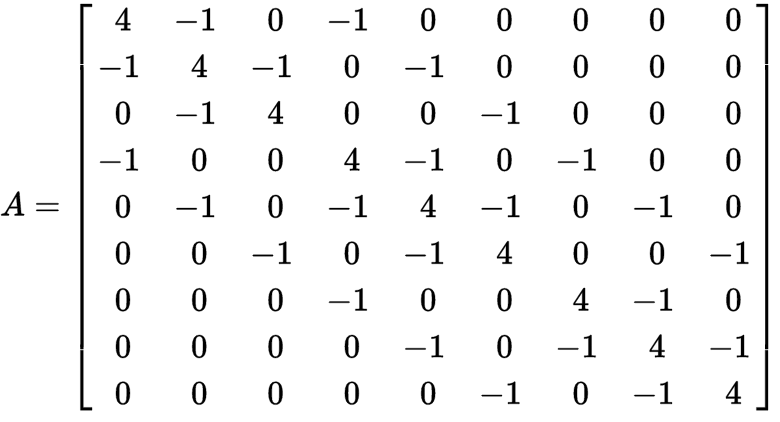
\includegraphics[width=0.5\textwidth]{poisson}
    \caption{An example of a tridiagonal matrix}
\label{fig:poisson}
\end{figure}
\noindent
Terrain generation is handled by a MatLab script. The whole process is pretty straightforward, once defined the resolution (512x512) a tridiagonal matrix (Figure~\ref{fig:poisson}) from \textit{Poisson's
discrete equation} is generated. Then the matrix is divided by another matrix of normally distributed random numbers, and converted to a gray-scale image. At this point a \textit{Gaussian blur} with $\sigma = 3
$is applied to the resulting image. An example is shown in Figure~\ref{fig:2dterrain}.

\subsection{Data postprocessing and Dataset Generation}
As what we obtain from the simulations is simply raw data, it needs to pass a post-processing phase. This phase is handled by a python script which parses each line of the
CSV generated from the simulations and produces a \textit{numpy} \cite{numpy} array of features and targets. \\
From each CSV record a patch is extracted, this patch (as Figure~\ref{fig:patch} shows) is not oriented by robot's yaw, so in order to rearrange it, the method \texttt{extract\_patch} was implemented.
First, a 2x3 transformation matrix is computed, then the computation is handled by an OpenCV method called \texttt{warpAffine}, which returns what is shown in Figure~\ref{fig:rpatch}.\\
From the oriented patch, the previously mentioned statistics are computed, then they are stored in a \textit{numpy} array as following: \\\\
\begin{longtabu}{| c | c | c | c | c | c | c |}
\rowfont{\bfseries}
\hline
    MEAN & VARIANCE & MEAN\_GRAD\_X & VAR\_GRAD\_X & MEAN\_GRAD\_Y & VAR\_GRAD\_Y & TRAVERSED \\
\hline
    \multicolumn{6}{ |c| }{DATA} & TARGET\\
\hline
    \rowcolor{LightGreen}
    1.20e+02 & 2.70e+03 & 2.73e+01 & 8.53e+02 & -1.03e+01 & 1.37e+03 & 1\\
    \rowcolor{LightGreen}
    1.14e+02 & 2.57e+03 & 2.83e+01 & 1.10e+03 & 1.16e+01 & 1.12e+03 & 1\\
    7.62e+01 & 1.37e+03 & 1.40e+01 & 1.15e+03 & 2.77e+00 & 1.16e+03 & 0\\
    9.98e+01 & 2.48e+03 & 3.01e+01 & 1.02e+03 & -5.73e+00 & 1.39e+03 & 0\\
    6.62e+01 & 9.96e+02 & 1.34e+01 & 1.37e+03 & -2.04e+00 & 8.25e+02 & 0\\
    \rowcolor{LightGreen}
    1.38e+02 & 1.25e+03 & 1.92e+01 & 9.69e+02 & -8.63e+00 & 8.67e+02 & 1\\
    1.25e+02 & 7.60e+02 & 1.44e+01 & 7.99e+02 & 4.93e+00 & 9.31e+02 & 0\\
    9.18e+01 & 1.45e+03 & 1.64e+01 & 1.09e+03 & -1.10e+01 & 1.03e+03 & 0\\
    1.14e+02 & 3.99e+02 & 9.33e+00 & 1.39e+03 & -3.21e+00 & 6.49e+02 & 0\\
    1.15e+02 & 4.54e+02 & 6.20e+00 & 7.77e+02 & 2.71e+00 & 8.70e+02 & 0\\
\hline
    \caption{An instance of the training dataset}
\end{longtabu}
\subsection{Training}
Training is handled by a python script which loads a dataset of 5000 samples and fits a classifier using \textit{logistic regression}.
\newpage
\section{Evaluation and Results}
In order to test the accuracy of the trained classifier we have computed some relevant statistics for the following linear methods:
\begin{itemize}
    \item Nearest Neighbor (with 3 as the number of neighbors)
    \item Support Vector Classificiation (with 3 different penalty parameters C=0.01, C=1, and C=100)
    \item Linear Support Vector Classification
    \item Logistic Regression
    \item Gaussian Naive Bayes
    \item a dummy classifier with a "most\_frequent" strategy (always predicts the most frequent label in the training set)
    \item a dummy classifier with a "stratified" strategy (generates predictions by respecting the training set's class distribution)
\end{itemize}
The script that handles the evaluation part, offers the possibility to apply \textit{cross validation} which is a technique used when working only with a unique dataset for both training
and testing, that prevents unpleasant mistakes such \textit{overfitting}, by taking a random split of the dataset for testing. \\
Following is presented an evaluation of our classifier for the previously mentioned methods using a different testing dataset.
\begin{longtabu}{| l | c | c |}
\rowfont{\bfseries}
    \hline
    METHOD & AUC & ACCURACY \\
    \hline
    KNeighborsClassifier(n\_neighbors=3) & 0.99 & 0.98 \\
    SVC(C=0.01) & 0.91 & 0.81\\
    SVC(C=1) & 0.95 & 0.90 \\
    SVC(C=100) & 0.98 & 0.97 \\
    LinearSVC(C=1.0) & 0.90 & 0.83 \\
    \rowcolor{LightCyan}
    LogisticRegression(C=1.0) & 0.96 & 0.93 \\
    GuassianNB() & 0.88 & 0.83 \\
    DummyClassifier('strategy=most\_frequent') & 0.50 & 0.69 \\
    DummyClassifier('strategy=stratified') & 0.49 & 0.57 \\
    \hline
\caption{Evaluation of each the classifier}
\label{table:datatest}
\end{longtabu}
\noindent
For each method we have computed both accuracy and \textit{auc} reaching good scores in estimations. Below is the graphic visualization of the ROC curve for the logistic regression method:
\begin{figure} [H]
\centering
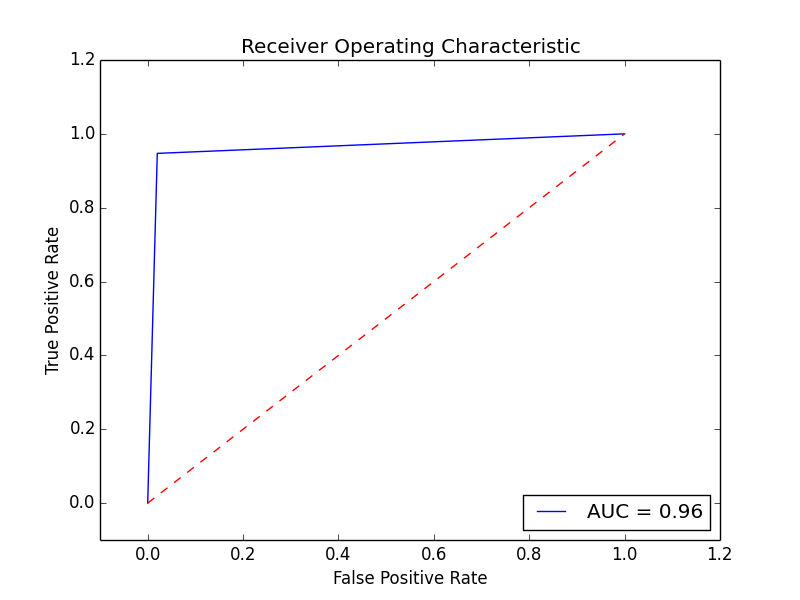
\includegraphics[width=0.6\textwidth]{roc_auc}
    \caption{The ROC curve using logistic regression}
\label{fig:roc_auc}
\end{figure}
\noindent
As traversability depends on the direction in which a terrain is traversed, we have tried to test how our classifier behaves, analyzing 8 different directions 
(0 to 360 by a step of 45 degrees). Following are two experiments on two different 10 x 10m heightmaps.\\
Each heightmap is represented as a 10x10 grid, so each cell has dimensions 1m x 1m; the classifier estimates runs of 2m, coloring each cell with green or red depending on a positive or
negative prediction.\\
The first heightmap contains an X-shaped tiny wall, while the second one represents a more realistic scenario.
\begin{figure}[H]
\minipage{0.48\textwidth}
  
\includegraphics[width=\linewidth]{x}
    \caption{The first tested heightmap: there's a tiny X wall inside it}\label{fig:x}
\endminipage\hfill
\minipage{0.48\textwidth}
  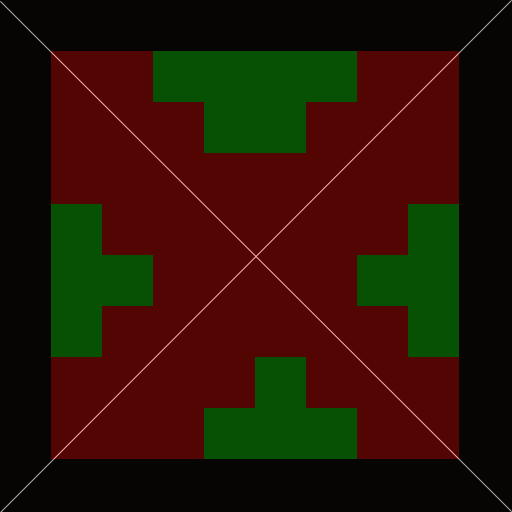
\includegraphics[width=\linewidth]{x90}
    \caption{the heightmap traversed in $\downarrow$ direction: the classifier estimates with accuracy traversable areas.}\label{fig:x90}
\endminipage\hfill
\end{figure}

\begin{figure}[H]
\minipage{0.32\textwidth}
  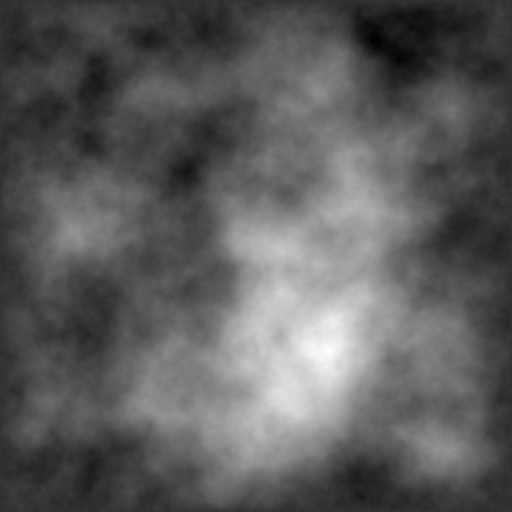
\includegraphics[width=\linewidth]{2dterrain}
    \caption{The second tested heightmap that represents outdoor environment}\label{fig:2dterrain}
\endminipage\hfill
\minipage{0.32\textwidth}
  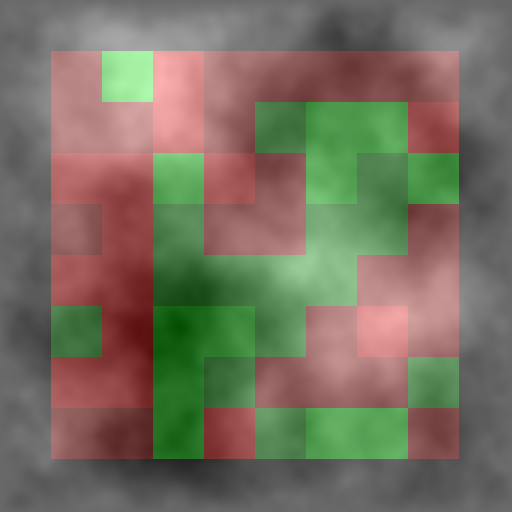
\includegraphics[width=\linewidth]{heatmap0}
    \caption{the heightmap traversed in $\rightarrow$ direction: here the classifier estimates correctly}\label{fig:heatmap0}
\endminipage\hfill
\minipage{0.32\textwidth}
  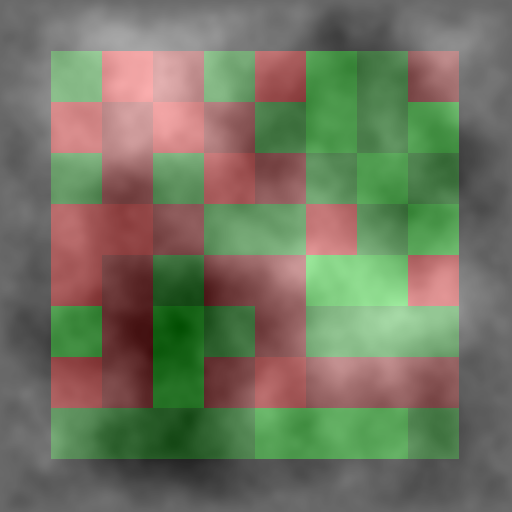
\includegraphics[width=\linewidth]{heatmap45}
    \caption{the heightmap traversed in $\searrow$ direction: as in the $\rightarrow$ case, the classifier does not estimate correctly green points on the diagonal}\label{fig:heatmap45}
\endminipage\hfill
\end{figure}



\begin{figure}[H]
\minipage{0.32\textwidth}
  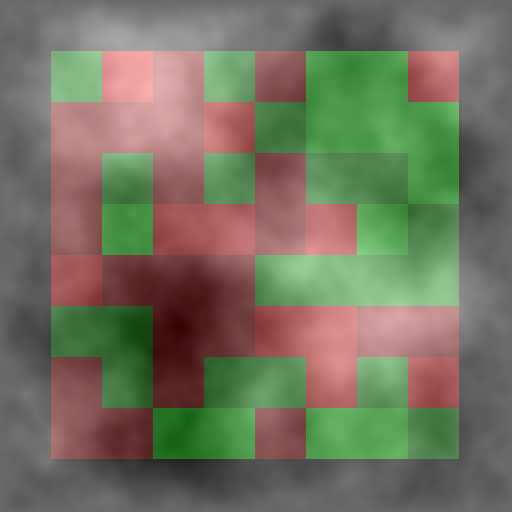
\includegraphics[width=\linewidth]{heatmap90}
    \caption{the heightmap traversed in $\downarrow$ direction: here the classifier estimates correctly }\label{fig:heatmap90}
\endminipage\hfill
\minipage{0.32\textwidth}
  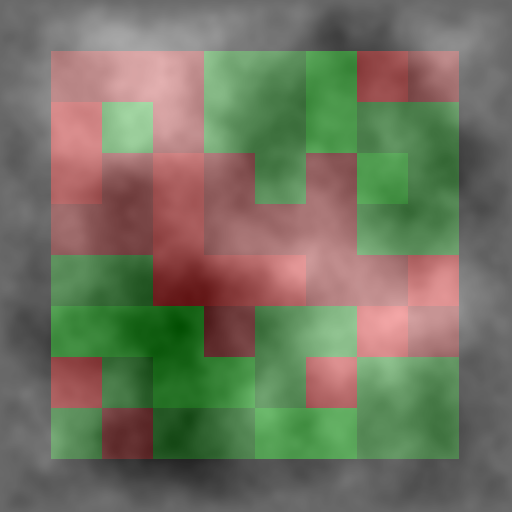
\includegraphics[width=\linewidth]{heatmap135}
    \caption{the heightmap traversed in $\swarrow$ direction: here the classifier estimates correctly}\label{fig:heatmap135}
\endminipage\hfill
\minipage{0.32\textwidth}
  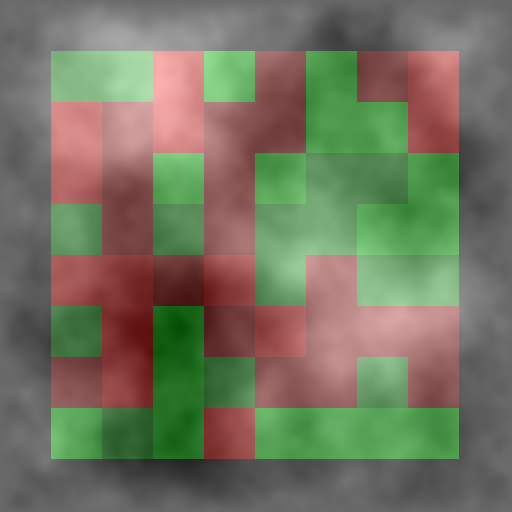
\includegraphics[width=\linewidth]{heatmap180}
    \caption{the heightmap traversed in $\leftarrow$ direction: as in the $\rightarrow$ case, the classifier does not estimate correctly green points on the diagonal}\label{fig:heatmap180}
\endminipage\hfill
\end{figure}


\begin{figure}[H]
\minipage{0.32\textwidth}
  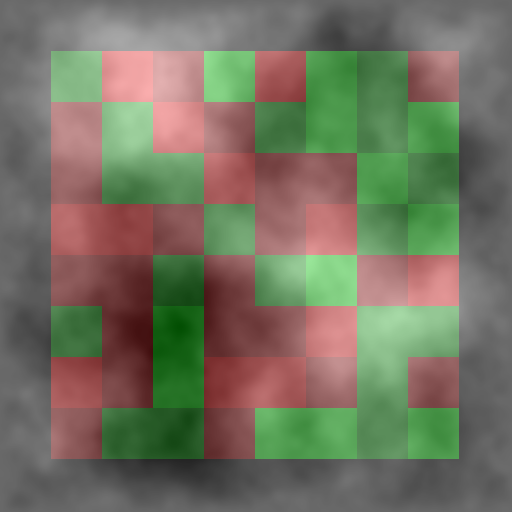
\includegraphics[width=\linewidth]{heatmap225}
    \caption{the heightmap traversed in $\nwarrow$ direction: as in the $\searrow$, the classifier misses 4 center patches}\label{fig:heatmap225}
\endminipage\hfill
\minipage{0.32\textwidth}
  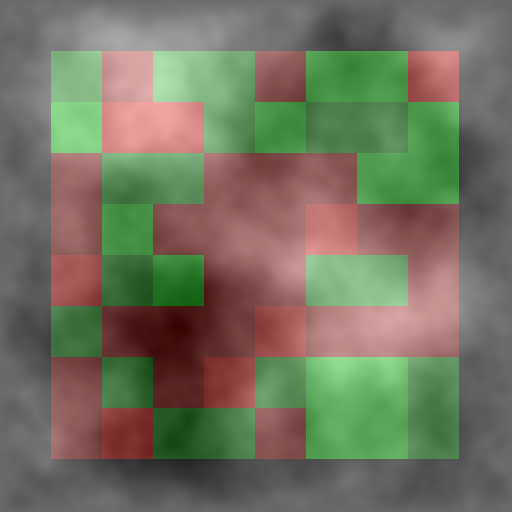
\includegraphics[width=\linewidth]{heatmap270}
    \caption{the heightmap traversed in $\uparrow$ direction: here the classifier estimates correctly}\label{fig:heatmap270}
\endminipage\hfill
\minipage{0.32\textwidth}
  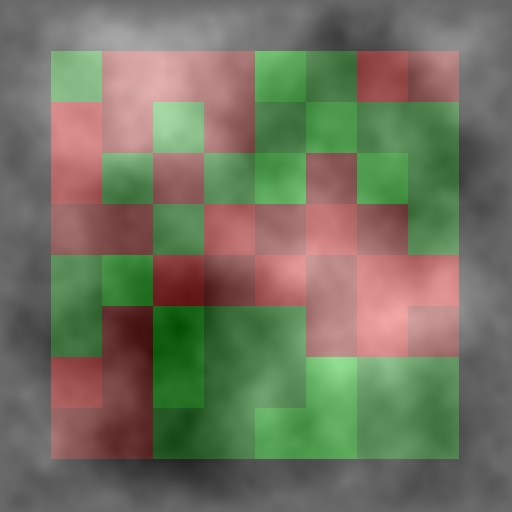
\includegraphics[width=\linewidth]{heatmap315}
    \caption{the heightmap traversed in $\nearrow$ direction: as in the $\swarrow$, the classifier estimates correctly}\label{fig:heatmap315}
\endminipage\hfill
\end{figure}

\newpage

\section{Conclusions and future work}
This thesis presents a first approach on path planning with no human intervention. The classifier, even if composed from simple features, predicts with optimal accuracy the traversability of a
given terrain, although more improvements in both data collection and learning can be done. \\
The main challenges in this work were the familiarization with the V-REP environment, (which like the majority of open source software, is constantly updated and does not have  a vast community 
of users), the implementation of the controller for the robot, and understanding the principles of machine learning.
Possible future research and work can be summed up in 4 different key parts:
\begin{itemize}
    \item
        extend the approach to more complex robot models, (legged robots). This will require our controller to integrate control of foothold stability, in order to perform
        reliable simulations, and some more accurate analysis on the terrain when training the classifier.
    \item
        validate the approach for real robots, meaning doing the actual testing phase in a real outdoor environment, with a real robot, but this may require more constraints,
        thinking about vegetation, rocks, and other obstacles that can be encountered.
    \item
        integrate the classifier's prediction in a path planning system, a task that will also require more study, especially in the decision making phase.
    \item
        investigate the possibility to apply the system in a real world environment with the help of stereo-imagery. In other words, using the knowledge obtain by the classifier on a large variety
        of terrains, together with a time of flight camera for obstacle detection, to perform navigation in rough terrains.
\end{itemize}
In addition, as suggested by \textit{Alessandro Giusti}, we are currently working in generating two datasets (both on the same terrain): one is obtained by running the robot at a normal speed, while
the other one travels at 3x speed. The purpose of this experiment is to analyze how a tune in robot mobility characteristics change the traversability of the same environment.

\subsection{Acknowledgments}
I want to thank my advisor and professor \textit{Luca Maria Gambardella} and my TAs \textit{Alessandro Giusti} and \textit{Jerome Guzzi} who have given me the opportunity to work on a really interesting and 
challenging project, and have helped and follow me during this whole semester. Another big thank goes to \textit{Vasileios Triglianos} who has helped me in the correction process of this report.

\newpage
%%%%%
\bibliographystyle{plain}
\bibliography{references}

\end{document}
